%!TEX root = ../report.tex

\begin{document}
    \chapter{基础功能}

    \section{顶点变换}
    \begin{spacing}{2.5}
    在软光栅渲染器中,顶点变换的基本任务是把空间三维顶点转换成屏幕上的二维坐标。这个过程涉及坐标变换的流水线,如图所示:\\
    \begin{figure}[H]
		\centering
		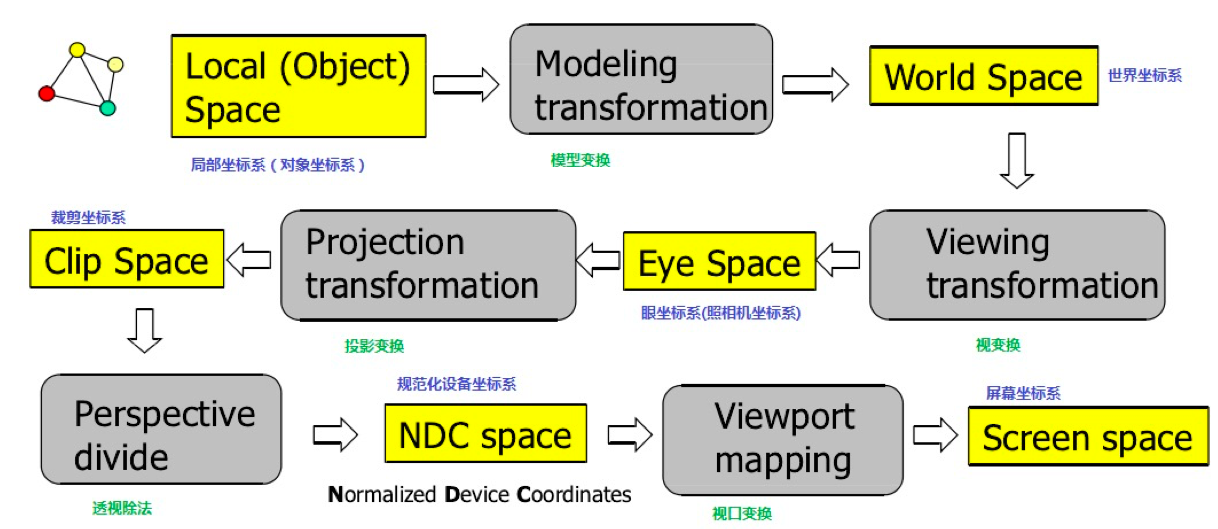
\includegraphics[width=1.0\textwidth]{images/pipline.png}
		\caption{软光栅渲染器坐标处理流水线}
		\label{line}
	\end{figure}
    \end{spacing}

    为了充分理解流水线各段,需要对几个坐标系进行理解。
    \subsection{局部坐标系}
    \begin{spacing}{2.5}
    每个物体在被创建时,都会有自己的局部坐标系,一般是以物体的几何中心为原点,那么物体的每个顶点相对于几何中心都会有一个相对坐标。这个坐标系就被称为物体的局部坐标系(Local Object Space)。该坐标系不是固定的,每个物体都有他们独立的坐标系,且仅对该对象适用。在物体移动或改变方向时,其局部坐标系也将随着移动或改变方向。
    \end{spacing}
    
    \subsection{世界坐标系}
    \begin{spacing}{2.5}
    因为每个物体都有自己的独立局部坐标系,如果要对多个物体观察,我们需要将它们放置到同一个绝对坐标系下,这个坐标系就叫世界坐标系(World Space)。世界坐标系始终是固定不变的。
    \end{spacing}
    
    \subsection{相机坐标系}
    \begin{spacing}{2.5}
    当我们在世界坐标系中对物体进行观察时,就会有一个观察原点,对应一个相机坐标系(Eye Space),相机坐标系是和观察者密切相关的坐标系。相机坐标系和屏幕坐标系相似,差别在于相机坐标系在三维空间中,而屏幕坐标系在二维平面里。为了方便处理,相机坐标系的原点和世界坐标系的原点是重合的,世界坐标系的z轴从相机的视角中心穿过。如图所示:
    \begin{figure}[H]
		\centering
		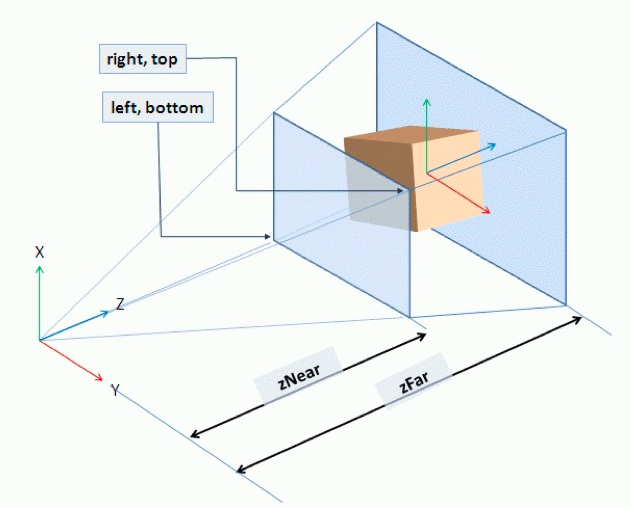
\includegraphics[width=0.8\textwidth]{images/camera.png}
		\caption{相机坐标系的原点与世界坐标系的原点重合}
		\label{camera}
	\end{figure}
    \end{spacing}
    
    \subsection{裁剪坐标系}
    \begin{spacing}{2.5}
    要了解为何要有裁剪坐标系,我们先得了解视锥体的概念:
    \subsubsection{视锥体}
    在图\ref{camera}中,相机有近视面zNear和远视面zFar,只有处在近视面和远视面中间的物体才能被相机所观测到,近视面和远视面共同将相机的视角切分成了一个锥体,这个锥体就叫做视锥体。\\ 
    \indent 正如我们前面所提,只有在视锥体中的物体才能被观测到,那么对物体处于视锥体外的部分自然要进行裁剪,但是在不规则的视锥体内进行裁剪是一件非常困难的事,所以人们将相机坐标投影到裁剪坐标系(Clip Space),裁剪坐标空间是一个立方体,这就很容易进行裁剪。
    \end{spacing}
    
    \subsection{规范化设备坐标系}
    \begin{spacing}{2.5}
    为了消除底层物理特性对裁剪的干扰,通常会把裁剪空间变换成一个规范化立方体,这个立方体的x,y,z坐标范围都是[-1,1]。这个坐标系被称为规范化设备坐标系(NDC space)。
    \end{spacing}
    
    \subsection{屏幕坐标系}
    \begin{spacing}{2.5}
    通常将屏幕上的设备坐标称为屏幕坐标。设备坐标又称为物理坐标,是指输出设备上的坐标。设备坐标用对象距离窗口左上角的水平距离和垂直距离来指定对象的位置,是以像素为单位来表示的,设备坐标的X轴向右为正,Y轴向下为正,坐标原点位于窗口的左上角。\\
    \end{spacing}
    
	了解了各个坐标系后,就能对各个坐标系的变换有更深的认识。
	\subsection{模型变换}
	\begin{spacing}{2.5}
		把物体从世界坐标系变换到局部坐标系称为模型变换。模型变换设计到的变换通常是很简单的平移变换。在我们的项目中味了进行简化,在创建物体时就给予了物体一个绝对坐标。三维空间中的平移变换矩阵如下:
		\begin{equation}
		\begin{pmatrix}
			1 &  0&  0&0 \\ 
 			0&  1&  0& 0\\ 
 			0& 0 & 1 &0 \\ 
 			T_{x}&  T_{y}&  T_{z}& 1
		\end{pmatrix}
		\label{transfer}
		\end{equation}
	\end{spacing}
	
	\subsection{视变换}
	\begin{spacing}{2.5}
	把物体从世界坐标变换到相机空间称为视变换,如前面所提,视变换主要是把物体通过平移和旋转变换到视锥体中,所以用到的变换主要是平移和旋转变换,平移变换矩阵为等式\ref{transfer},旋转变换矩阵为:
	\end{spacing}
	\begin{itemize}
	\item 绕Y轴旋转
	\begin{equation}
		\begin{pmatrix}
			cos\theta &  0&  -sin\theta &0 \\ 
 			0&  1&  0& 0\\ 
 			sin\theta & 0 & cos\theta &0 \\ 
 			0&  0&  0& 1
		\end{pmatrix}
		\label{xrotate}
	\end{equation}
	\item 	绕X轴旋转
	\begin{equation}
		\begin{pmatrix}
			 1&  0&  0 &0 \\ 
 			0&  cos\theta &  sin\theta& 0\\ 
 			 0& -sin\theta & cos\theta &0 \\ 
 			0&  0&  0& 1
		\end{pmatrix}
		\label{yrotate}
		\end{equation}
	\item 绕Z轴旋转
	\begin{equation}
		\begin{pmatrix}
			cos\theta &  sin\theta &  0 &0 \\ 
 			-sin\theta &  cos\theta &  0& 0\\ 
 			0 & 0 & 1 &0 \\ 
 			0&  0&  0& 1
		\end{pmatrix}
		\label{zrotate}
	\end{equation}
	\end{itemize}
	
	
	\subsection{投影变换}
	\begin{spacing}{2.5}
	从相机坐标系到裁剪坐标系的变换称为投影变换。投影变换矩阵的推导如下:
	\end{spacing}
		先观察视锥体的一个截面,如图所示:
		\begin{spacing}{2.5}
		\begin{figure}[H]
		\centering
		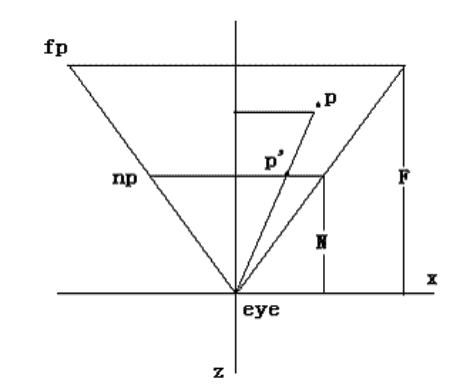
\includegraphics[width=0.5\textwidth]{images/project1.png}
		\caption{视锥体截面}
		\label{project1}
	\end{figure}
	图中$N$是观察原点到近视面的距离,$F$是观察原点到远视面的距离,$P(x,y,z)$为视锥体中的点,$P^{'}(x^{'},y^{'},z^{'})$是投影之后的点。这里z轴指向视锥体的反方向,指向正方向的推导过程与之类似。投影面可以选择任何平行于近视面的平面,为了简化分析,这里我们选择近视面作为投影平面。于是有$z^{'}=-N$,通过相似三角形容易得到以下式子:
	\begin{equation}
	\begin{split}
		\frac{x}{x^{'}}=\frac{z}{z^{'}}=\frac{z}{-N} \\
		x^{'} = -N\frac{x}{z} \\
		y^{'} = -N\frac{y}{z}
		\label{project_1}
	\end{split}
	\end{equation}
	这样$P^{'}$可以写为:
	\begin{equation}
		P^{'}=(-N\frac{x}{z},-N\frac{y}{z},-N)
	\end{equation}
	正如我们前面提到的,在不规则视锥体中进行裁剪是一件非常麻烦的事情,因此需要一个规范化的裁剪空间(CVV),假定裁剪空间中$x,y,z\in[-1,1]$,因此我们构造z的一个映射:
	\begin{equation}
	z^{'}=-\frac{az+b}{z}
	\label{project_2}
	\end{equation}
	使得式子 Eq.\ref{project_2} 在$z=-N$时的值为-1,而在$z=-F$时的值为1。于是投影变换可以暂时写为:
	\begin{equation}
		\begin{pmatrix}
		N & 0 & 0 &0 \\ 
		0 & N & 0 &0 \\ 
		0 & 0 & a &b \\ 
		0 & 0 & -1 &0 
	\end{pmatrix}\begin{pmatrix}
	x\\ 
	y\\ 
	z\\ 
	1
	\end{pmatrix}=\begin{pmatrix}
	-Nx/z\\ 
	-Ny/z\\ 
	-(az+b)/z\\ 
	1
	\end{pmatrix}
		\label{project_3}
	\end{equation}
	由待定系数法,有:
	\begin{equation}
		\begin{split}
			-\frac{az+b}{z}=
		\left\{\begin{matrix}
		-1, & if & z = -N\\ 
		1, & if & z = -F
		\end{matrix}\right.
		\end{split}
	\end{equation}
	可以计算出系数$a,b$:
	\begin{equation}
		\begin{split}
			a = -\frac{F+N}{F-N} \\
			b = -\frac{2FN}{F-N}
		\end{split}
	\end{equation}
	代入式子 Eq.\ref{project_3}这样就可以得到透视投影矩阵的第一个版本:
	\begin{equation}
		\begin{pmatrix}
		N & 0 & 0 &0 \\ 
		0 & N & 0 &0 \\ 
		0 & 0 & -\frac{F+N}{F-N} &\frac{-2FN}{F-N} \\ 
		0 & 0 & -1 &0 
	\end{pmatrix}
	\label{project_4}
	\end{equation}
	虽然z方向满足CVV的要求了,但是x,y方向仍没有被限制在$[-1,1]$之间,我们将投影平面的左边界值记为$left$,右边界值记为$right$,即$[left,right]$,同理对上下边界有$[bottom,top]$。要把$-Nx/z\in[left,right]$和$-Ny/z\in[bottom,top]$映射到$[-1,1]$中,需要用到线性插值:
	\begin{equation}
		\begin{split}
		\left\{\begin{matrix}
		\frac{-Nx/z-left}{right-left}=\frac{x-(-1)}{1-(-1)}\\ 
		\frac{-Ny/z-bottom}{top-bottom} = \frac{y-(-1)}{1-(-1)}
		\end{matrix}\right.
		\end{split}
	\end{equation}
	可以解得:
	\begin{equation}
		\begin{split}
		\left\{\begin{matrix}
		x=\frac{-2Nx/z}{right-left}-\frac{right+left}{right-left}\\ 
		y=\frac{-2Ny/z}{top-bottom} - \frac{top+bottom}{top-bottom}
		\end{matrix}\right.
		\end{split}
	\end{equation}
	于是,$P^{'}$可以再写为:
	\begin{equation}
		P^{'}=\begin{pmatrix}
		\frac{-2Nx/z}{right-left}-\frac{right+left}{right-left}\\ 
		\frac{-2Ny/z}{top-bottom} - \frac{top+bottom}{top-bottom}\\ 
		-(az+b)/z\\ 
		1
	\end{pmatrix}
	\end{equation}
	可以改写成:
	\begin{equation}
		P^{'}=\begin{pmatrix}
		\frac{2Nx}{right-left}+\frac{right+left}{right-left}z\\ 
		\frac{2Ny}{top-bottom} + \frac{top+bottom}{top-bottom}z\\ 
		az+b\\ 
		-z
	\end{pmatrix}
	\end{equation}
	设投影矩阵为M,则运用待定系数法有:
	\begin{equation}
	M\begin{pmatrix}
		x\\ 
		y\\ 
		z\\ 
		1
	\end{pmatrix}=\begin{pmatrix}
		\frac{2Nx}{right-left}+\frac{right+left}{right-left}z\\ 
		\frac{2Ny}{top-bottom} + \frac{top+bottom}{top-bottom}z\\ 
		az+b\\ 
		-z
	\end{pmatrix}
	\end{equation}
	可以求得矩阵M:
	\begin{equation}
		\begin{pmatrix}
		\frac{2N}{right-left} & 0 & \frac{right+left}{right-left} &0 \\ 
		0 & \frac{2N}{top-bottom} & \frac{top+bottom}{top-bottom} &0 \\ 
		0 & 0 & -\frac{F+N}{F-N} &\frac{-2FN}{F-N} \\ 
		0 & 0 & -1 &0 
	\end{pmatrix}
	\label{M}
	\end{equation}
	在实际应用中,更常使用视角$Fovy$和投影面的宽高比$Aspect$来进行投影变换矩阵的描述,$Fovy$和$N、F、left、right、top、bottom$的关系如图所示:
	\begin{figure}[H]
		\centering
		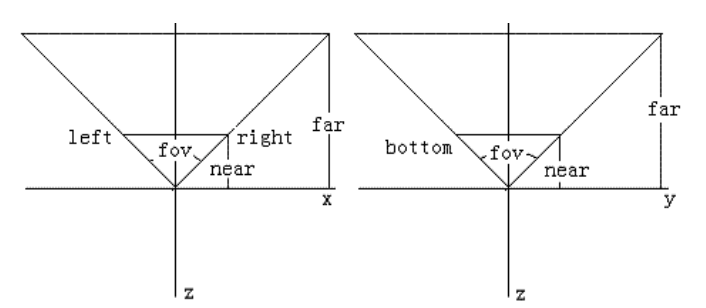
\includegraphics[width=0.7\textwidth]{images/fovy.png}
		\caption{视角Fovy示意图}
		\label{fovy}
	\end{figure}
	$Fovy$即视野,是视锥体在xz平面或者yz平面的开角角度。在OpenGL中使用yz平面。由图\ref{fovy}可以得到如下关系:
	\begin{equation}
		\begin{split}
			right = N \times tan(fovy/2)\\
			left = -right\\
			top = N \times tan(fovy/2)\\
			bottom = -top 
		\end{split}
		\label{fovy_1}
	\end{equation}
	而
	\begin{equation}
	Aspect = \frac{right-(-right)}{top-(-top)} = \frac{right}{top}
	\label{aspect}
	\end{equation}
	将式子 Eq.\ref{fovy_1} 和式子 Eq.\ref{aspect} 代入式子 Eq.\ref{M} 可得最终的投影矩阵M:
	\begin{equation}
		\begin{pmatrix}
		\frac{cot\frac{Fovy}{2}}{Aspect} & 0 &0 &0 \\ 
		0 & \frac{Fovy}{2} & 0 &0 \\ 
		0 & 0 & -\frac{F+N}{F-N} &\frac{-2FN}{F-N} \\ 
		0 & 0 & -1 &0 
	\end{pmatrix}
	\label{M_1}
	\end{equation}
	\end{spacing}
	
	\subsection{透视除法}
	\begin{spacing}{2.5}
	透视除法将裁剪坐标空间变换为NDC空间,方法如下:
	\begin{equation}
		\begin{pmatrix}
		x\\ 
		y\\ 
		z\\ 
		w
	\end{pmatrix}/w=\begin{pmatrix}
		x/w\\ 
		y/w\\ 
		z/w\\ 
		1
	\end{pmatrix}
	\end{equation}
	\end{spacing}
	\subsection{视口变换}
	\begin{spacing}{2.5}
	最后一个变换为视口变换,它将NDC空间变换到最终屏幕坐标系,视口变换矩阵的推导过程如下:
	视口变换是将下面立方体中的物体变换到视口即屏幕中:
	\begin{figure}[H]
		\centering
		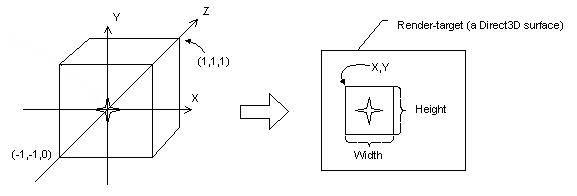
\includegraphics[width=0.8\textwidth]{images/viewport.png}
		\caption{视口变换示意图}
		\label{viewport}
	\end{figure}
	其中,立方体的坐标范围为:
	\begin{equation}
		\begin{split}
		\left\{\begin{matrix}
		-1\leq x\leq 1\\ 
		-1 \leq y \leq 1\\
		0 \leq z \leq 1
		\end{matrix}\right.
		\end{split}
	\end{equation}
	而视口的坐标范围是:
	\begin{equation}
		\begin{split}
		\left\{\begin{matrix}
		X \leq x\leq X + Width\\ 
		Y \leq y \leq Y + Height\\
		MinZ \leq z \leq MaxZ
		\end{matrix}\right.
		\end{split}
	\end{equation}
	在图\ref{viewport}中,视口的起点为$(X,Y)$,宽高分别为$Width$和$Height$,x轴向右为正,y轴向下为正,y轴的方向与三维坐标正好相反。视口是一个2D平面,在视口变换中,Z坐标也是跟着变换的,只是在图中没有体现。
	假设变换矩阵的第一列为$[x^{'},y^{'},z^{'},1]^{T}$,根据上图,立方体在(-1,1,0,1)映射到视口中的起点(X,Y,MinZ,1),立方体中的右上角点(1,1,0,1)映射到视口中的点(X+Width,Y,MinZ,1),于是可以列式:
	\begin{equation}
	\begin{split}
		\left\{\begin{matrix}
		[-1,1,0,1]*[x^{'},y^{'},z^{'},1]^{T} = X\\ 
		[1,1,0,1]*[x^{'},y^{'},z^{'},1]^{T} = X+Width\\
		\end{matrix}\right.
		\end{split}
	\end{equation}
	可以求得变换矩阵的第一列:$$[\frac{Width}{2},0,0,x+\frac{Width}{2}]$$
	同理可以求得变换矩阵的第二列、第三列、第四列,从而可以求得视口变换矩阵:
	\begin{equation}
		\begin{pmatrix}
		\frac{Width}{2} & 0 &0 &0 \\ 
		0 & -\frac{Height}{2} & 0 &0 \\ 
		0 & 0 & MaxZ-MinZ & 0 \\ 
		X+\frac{Width}{2} &Y+\frac{Height}{2} & MinZ &1 
	\end{pmatrix}
	\end{equation}
	通常的视口坐标系的起点为$[X,Y]=[0,0]$,我们也不需要关注Z方向上的变换。
	\end{spacing}
    \section{裁剪}
    \section{线框画线}
    \begin{spacing}{2.5}
    光栅中常用的算法仍是Bresenham算法,我们的项目也一样。关于Bresenham算法的原理课堂上已经有详细的描述,此处不再赘述。书本上对Bresenham算法的描述限制在$x > 0, y > 0$且直线斜率在$[0,1]$之间,即下图中的1a象限:
    \begin{figure}[H]
		\centering
		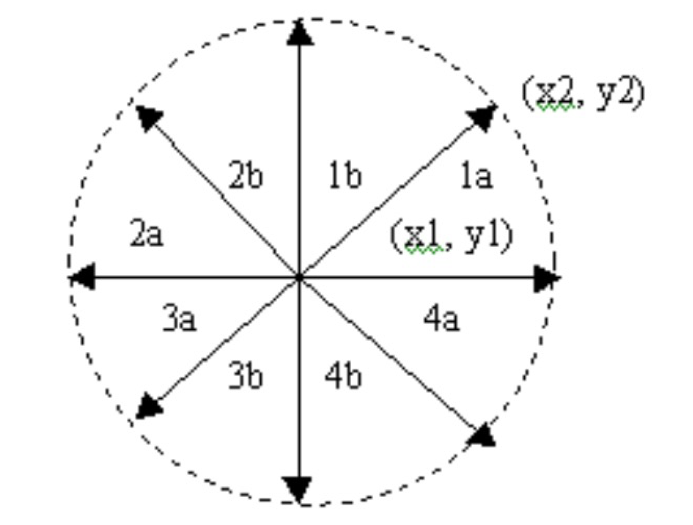
\includegraphics[width=0.5\textwidth]{images/block.png}
		\caption{Bresenham画线象限示意图}
		\label{block}
	\end{figure}
	为了实现光栅渲染,必须将Bresenham扩展到全部8个象限。其实其他象限的基本处理思路与1a是一样的,只不过在1a中y随x递增而递增,在其他象限可能是x随y递增而递增,y随x递增而递减,具体情况如下表所示,只需要判定当前属于哪一象限,然后相应使用Bresenham即可。
	\begin{table}[H]
	\begin{center}
    \begin{tabular}{p{5cm}|p{5cm}}
        \hline
        象限 & 取值\\
        \hline
        1a、2a &  $y_{i+1}=y_{i}$或$y_{i} = y_{i}+1$\\
        \hline
        3a、4a & $y_{i+1}=y_{i}$或$y_{i} = y_{i}-1$\\
        \hline
        1b、2b & $x_{i+1}=x_{i}$或$x_{i} = x_{i}+1$\\
        \hline
        3b、4b & $x_{i+1}=x_{i}$或$x_{i} = x_{i}-1$\\
        \hline
    \end{tabular}
	\end{center}
	\caption{象限取值表}
	\end{table}
    \end{spacing}
\end{document}
